\documentclass{article}
\usepackage[utf8]{inputenc}
\usepackage{graphicx}
\usepackage{color}
\usepackage{float}
\usepackage{geometry}
\definecolor{orange}{rgb}{0.99,0.50,0.07}
\definecolor{color2}{rgb}{0.0,0.0,0.0}



\geometry{top=55, bottom=55,left=50 ,right=50}

\begin{figure}
\hspace{155}

\includegraphics[scale=0.1]{logo_TNCY.png}
\label{fig:logo_tncy}
\end{figure}

\title{\bf \color{orange} RAPPORT de Projet}
\author{\color{color2} Camille COUÉ , Victor COUR , Erwan KESSLER}
\date{\it December 2018}

\begin{document}

\maketitle


\title{\bf \Large \color{orange} Sommaire}
\begin{itemize}
    \color{color2}
    \item Introduction
    \item L'organisation pour répartir le travail 
    \item Gestion des étapes
    \item Production finale : Étape 8
    \item Ce que le projet a apporté à chacun
    \item Remerciements
    \item Sources
\end{itemize}
\color{orange} \section { Introduction }

\color{color2}

Le but du projet est de créer un code qui permettrait de choisir la représentation (parmi celles qui sont proposées) où l’on placerait les différents aéroports du monde que le site openflight.org a rescencé en 2017. On pourrait aussi choisir de centrer cette représentation sur une zone souhaitée.

\vspace{1\baselineskip}

Nous avons profité du lendemain de l’annonce du projet pour nous donner rendez-vous dans un restaurant afin de faire connaissance. Après avoir défini l’heure de notre première réunion pour fixer l’organisation du projet , Erwan nous a suggérer de créer un Trello (plateforme visant à la gestion de version de projet) en attendant que la plateforme Git soit configurée.

\vspace{1\baselineskip}

\color{orange} \section{ L'organisation pour répartir le travail }

\color{color2}

Nous avons décidé pour hiérarchiser notre équipe de définir un chef de projet et nous avons convenu que Erwan remplirait ce poste.
Ainsi, Camille et Victor joueront les rôles de secrétaires pour rédiger les comptes rendus à tour de rôle. (Listes des comptes rendus en annexe)

\vspace{1\baselineskip}

La première étape pour se répartir le travail a été de prévoir la durée des tâches, nous avons d’abord effectué un GANTT prévisionnel pour avoir une idée des étapes les plus coûteuse en temps, et à l’inverse, celles qui n’en demandaient pas énormément.

\vspace{1\baselineskip}

\begin{figure}[H]
    \centering
    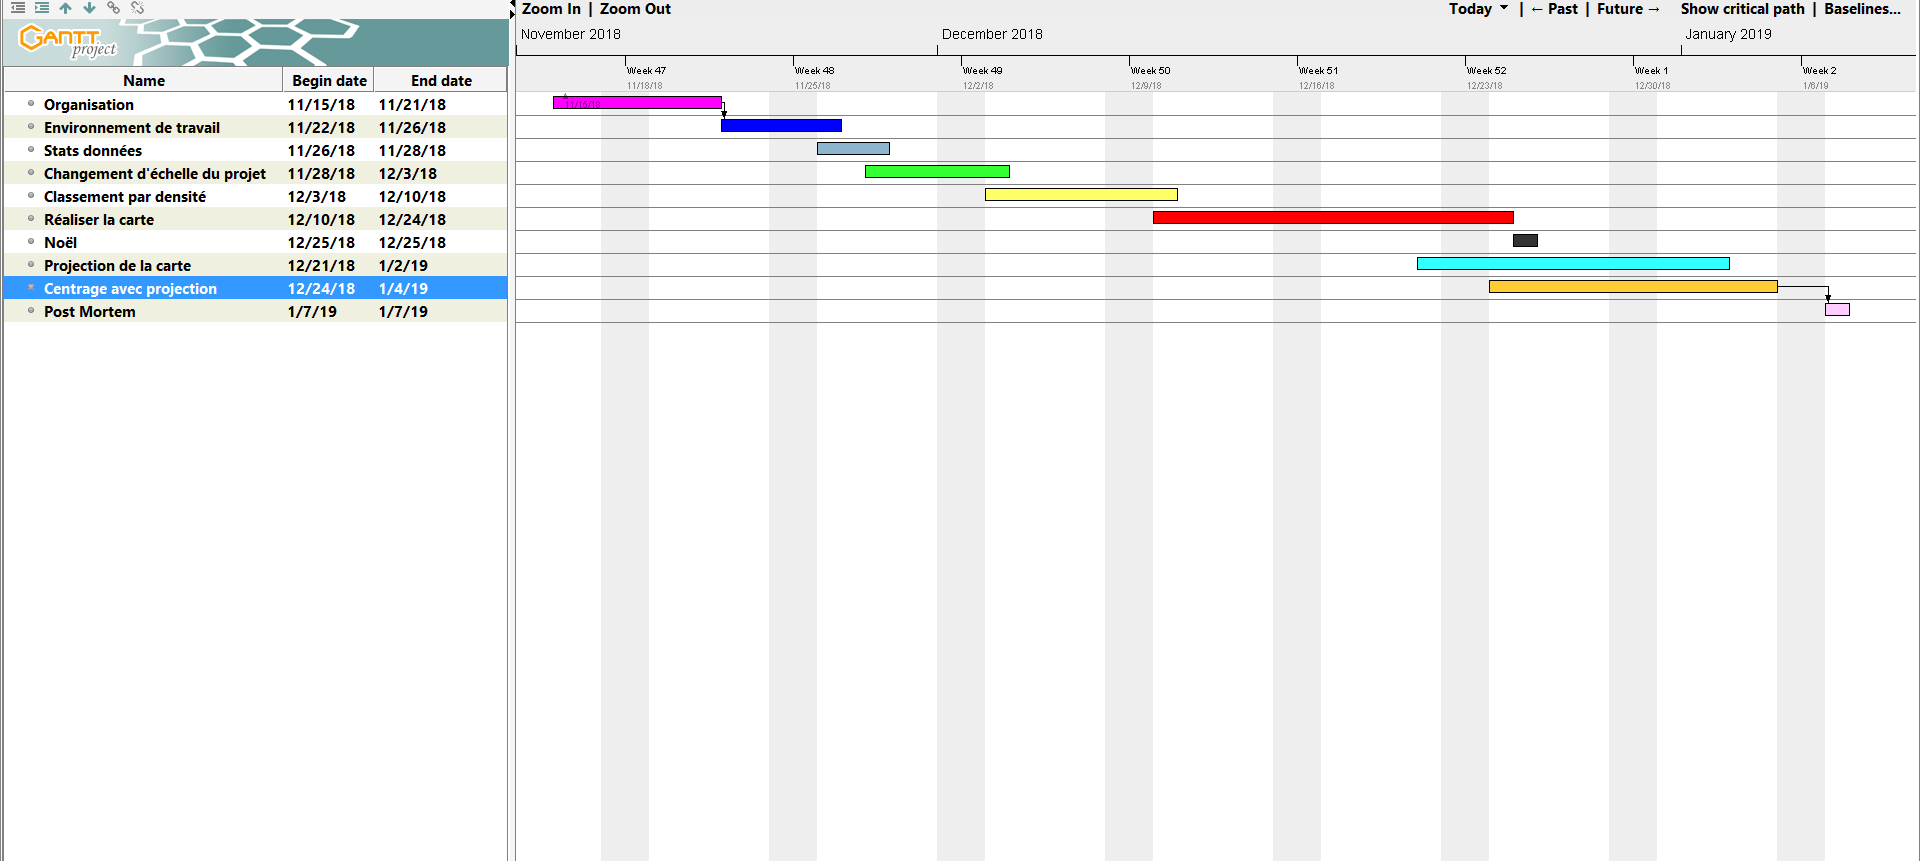
\includegraphics[scale=0.3]{gantt.png}
    \caption{Gantt prévisionnel}
    \label{fig:gantt}
\end{figure}

Nous avons ensuite réparti les tâches avec un responsable pour chacune d’entre elles grâce à une matrice RACI.

\vspace{1\baselineskip}

\begin{figure}[H]
    \centering
    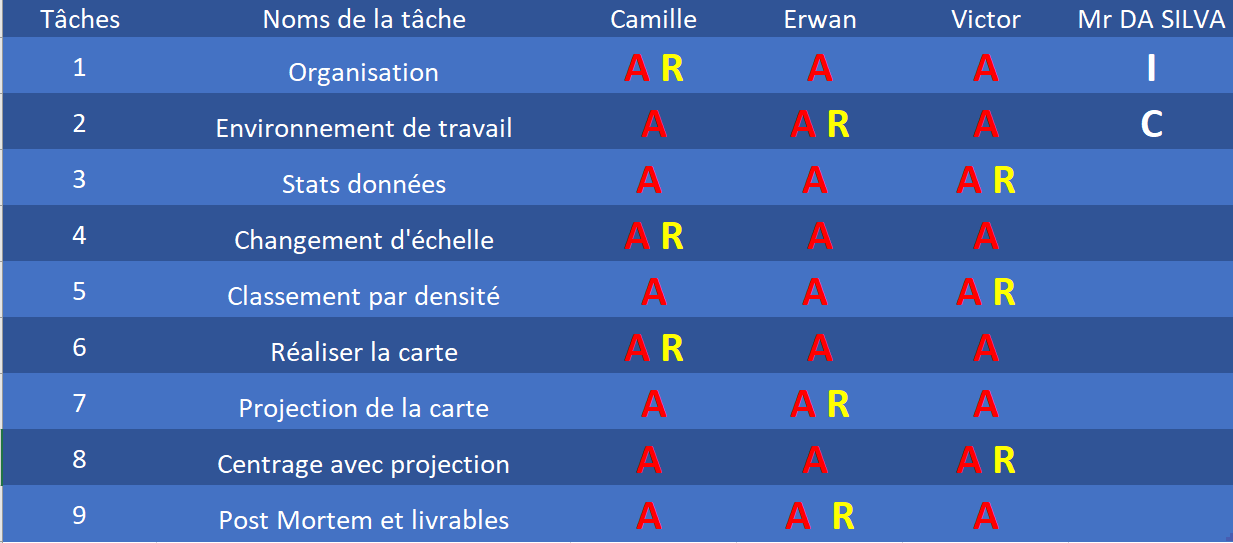
\includegraphics[scale=0.4]{raci.png}
    \caption{Matrice RACI}
    \label{fig:raci}
\end{figure}

Enfin, il ne restait plus qu’à prévoir les risques possibles dans le déroulement du projet, c’est pourquoi nous avons utilisé une matrice SWOT pour rendre compte des différents facteurs pouvant nous faire gagner du temps, ou nous en faire perdre.

\vspace{1\baselineskip}

\begin{figure}[H]
    \centering
    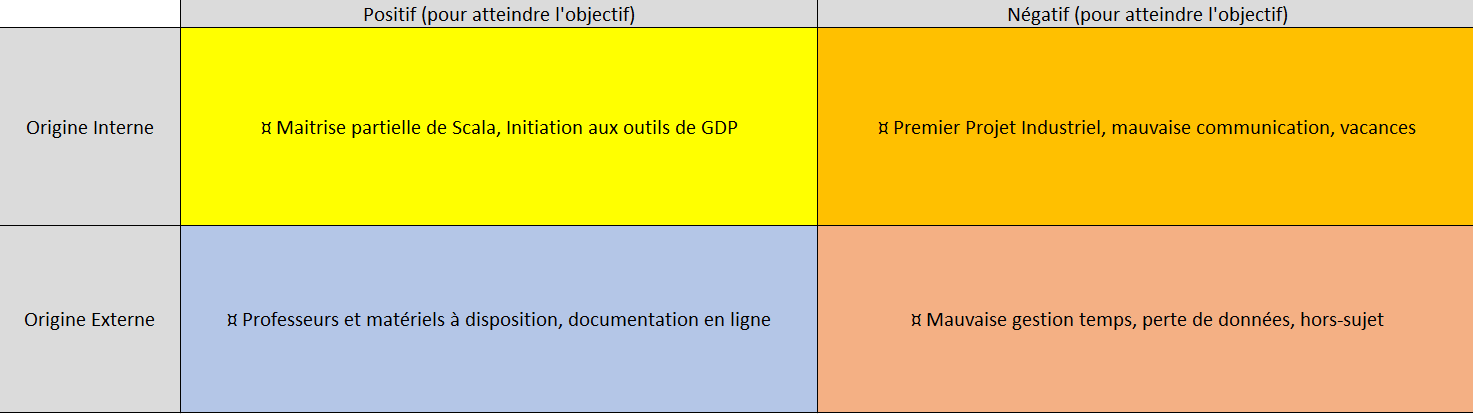
\includegraphics[scale=0.5]{swot.png}
    \caption{Matrice SWOT}
    \label{fig:swot}
\end{figure}

\vspace{3\baselineskip}

\color{orange} \section{ Gestion des étapes}


\subsection{ Étape 1} 
\color{color2}

\textbf{Problème rencontré :} \newline
Au premier abord, nous voulions lire le fichier ligne par ligne, et séparer les éléments de ces lignes par des virgules, cependant, il existait des chaînes de caractères possédant des virgules, empêchant la bonne séparation des éléments.

\vspace{1\baselineskip}

\noindent{\textbf{Solution :}} \newline
Suite au problème de séparation des éléments ligne par ligne, il a fallu trouver une expression régulière permettant d’écarter ce problème de virgules en donnant une séparation avec “,” ou “,\textbackslash{} ou encore “,[0-9] qui permettrait de gérer les conflits rencontrés avec les chaînes de caractères possédant des virgules.


\color{orange}
\subsection{Étape 2} 
\color{color2}

\textbf{Problème rencontré :} \newline
Plusieurs calculs permettant de mesurer une distance existent, l’objectif était de sélectionner la méthode donnant la distance la plus précise possible mais aussi la moins coûteuse en calcul.

\vspace{1\baselineskip}

\noindent{\textbf{Solution :}} \newline
Nous avons alors implémenter plusieurs des méthodes que nous avions trouvées en nous documentant. En testant sur nos données, nous avons remarqué que la méthode d'Harversine était la plus rapide et en plus, la plus précise. Nous avons donc choisi de l'utiliser dans la suite de notre travail. 

\color{orange}
\subsection{Étape 3} 
\color{color2}

\textbf{Problème rencontré :} \newline
Dans les statistiques, plusieurs méthodes permettaient de calculer la médiane grâce à notre structure de données. Il fallait donc, comme dans l'étape précédante, choisir la "bonne" méthode.

\vspace{1\baselineskip}

\noindent{\textbf{Solution :}} \newline
Ici aussi nous avons selectionné plusieurs méthodes et ensuite testé sur nos données. Nous avons choisi dans un premier temps d'utiliser la fonction .sorted pour trier le tableau, pour ensuite prendre l'élément au milieu (la médiane). Cependant, nous avons cherché pour voir s'il y avait une meilleure méthode que le .sorted, et Erwan a suggeré d'utiliser la méthode du quick select pour trier les données. Il est avéré qu'elle était plus rapide que .sorted.

\color{orange}
\subsection{Étape 4} 
\color{color2}

Pas de problème particulier sur cette étape.

\color{orange}
\subsection{Étape 5}
\color{color2}

\textbf{Problème rencontré :} \newline
 Nous avons convenu au départ de compter le nombre d'aéroports dans chaque pays en parcourant notre tableau et en mettant ce résultat dans un autre tableau (avec pour chaque case du tableau un pays lui étant associé). Cependant, il était compliqué d'attribuer un nombre pour chaque pays : la liste des identifiants de "airports.dat" n'étant pas des nombres consécutifs à chaque fois... 
 
\vspace{1\baselineskip}

\noindent{\textbf{Solution :}} \newline
Nous avons décidé d'utiliser les HashMap de la bibliothèque scala.collection.mutable car les HashMap permettent de créer un moyen plus pratique pour accéder aux données que l'on souhaite avoir sous la main. Il faut donc déjà parcourir une fois notre tableau de données pour créer cette HashMap, cependant on accède aux éléments avec une complexité en \textit{O}(1).

\vspace{1\baselineskip}
\color{orange}
\subsection{Étape 6} 
\color{color2}

\textbf{Problème rencontré :} \newline
L'image wrapper ne fonctionnait pas sur notre version de scala (2.12.7) et les versions supportées étaient "2.9.2", "2.10.6" et "2.11.7".

\vspace{1\baselineskip}

\noindent{\textbf{Solution :}} \newline
Pour régler ce problème de version pour l'image wrapper nous avons décider de regarder sur GitHub pour trouver une version adéquate. (Lien dans la partie Sources)

\color{orange}
\subsection{Étape 7}
\color{color2}

\textbf{Problème rencontré :} \newline
Après s'être documenté sur les projections conformes et équivalentes, il fallait transformer un couple (latitude,longitude) en (x,y) avec (x,y) les coordonnées dans la projection voulue. Cependant nous avons remarqué qu'il fallait faire une transformation linéaire sur ces coordonnées pour les placer au bon endroit dans notre image bitmap. Comment trouver ces transformations linéaires?

\vspace{1\baselineskip}
\noindent{\textbf{Solution :}}




\color{orange} \section{ Production finale : Étape 8}
\color{color2}

\color{orange} \section{ Ce que le projet a apporté à chacun}
\color{color2}

Voici tout d'abord le tableau des heures passées sur le projet :

\begin{figure}[H]
    \centering
    \includegraphics[scale=0.5]{}
    \caption{Table des heures de travail}
    \label{fig:tableheures}
\end{figure}


\color{orange} \section{ Remerciements}
\color{color2}

\begin{itemize}
    \color{color2}
    \item Nous souhaitons remercier l’ensemble de l’équipe pédagogique de Telecom Nancy pour nous avoir enseigné les méthodes et outils indispensable à la réalisation de notre projet.
    \item Plus particulièrement Mr DA SILVA (responsable du projet) et Mme HEURTEL ainsi que Rémi BACHELET pour la gestion de projet.
    \item Nous remercions également Telecom Nancy, pour avoir mis à notre disposition les infrastructures et le matériel informatique nécessaires au projet.
    \end{itemize}

\color{orange} \section{ Sources }
\color{color2}

\begin{itemize}
    \color{color2}
    \item
    \item
    \item
    \item
    \item
    \item
    \end{itemize}


\end{document}
